%%%%%%%%%%%%%%%%%%%%%%%%%%%%%%%%%%%%%%%%%%%%%%%%%%%%%%%%%%%%%%%%%%%%%%%%%%%%%%%%%%%%%%%%%%%%%%%%%%%
%%%%%%%%%%%%%%%%%%%%%%%%%%%%%%%%%%%%%%%%%%%%%%%%%%%%%%%%%%%%%%%%%%%%%%%%%%%%%%%%%%%%%%%%%%%%%%%%%%%
%%%%%%%%%%%%%%%%%%%%%%%%%%%%%%%%%%%%%%%%%%%%%%%%%%%%%%%%%%%%%%%%%%%%%%%%%%%%%%%%%%%%%%%%%%%%%%%%%%%
\documentclass[12pt,dvipdfmx]{beamer}
%%%%%%%%%%%%%%%%%%%%%%%%%%%%%%%%%%%%%%%%%%%%%%%%%%%%%%%%%%%%%%%%%%%%%%%%%%%%%%%%%%%%%%%%%%%%%%%%%%%%%%
% pdfの栞・プロパティの字化けを防ぐ
\usepackage{atbegshi}
%\AtBeginShipoutFirst{\special{pdf:tounicode 90ms-RKSJ-UCS2}} %Windows
\AtBeginShipoutFirst{\special{pdf:tounicode EUC-UCS2}} %Linux, Mac
\usepackage{hyperref}
%%%%%%%%%%%%%%%%%%%%%%%%%%%%%%%%%%%%%%%%%%%%%%%%%%%%%%%%%%%%%%%%%%%%%%%%%%%%%%%%%%%%%%%%%%%%%%%%%%%%%%
%%%
%%% テーマの指定、省略時は default になる
%%%

 % フレームの指定、省略可
%%%%%%%%%%%%%%%%%%%%%%%%%%%% THEME
  %\usetheme{AnnArbor}
  %\usetheme{Antibes}
  %\usetheme{Bergen}
  %\usetheme{Berkeley}
  %\usetheme{Berlin}
  \usetheme{Boadilla}
  %\usetheme{boxes}
  %\usetheme{CambridgeUS}
  %\usetheme{Copenhagen}
  %\usetheme{Darmstadt}
  %\usetheme{default}
  %\usetheme{Dresden}
  %\usetheme{Frankfurt}
  %\usetheme{Goettingen}
  %\usetheme{Hannover}
  %\usetheme{Ilmenau}
  %\usetheme{JuanLesPins}
  %\usetheme{Luebeck}
  %\usetheme{Madrid}
  %\usetheme{Malmoe}
  %\usetheme{Marburg}
  %\usetheme{Montpellier}
  %\usetheme{PaloAlto}
  %\usetheme{Pittsburgh}
  %\usetheme{Rochester}
  %\usetheme{Singapore}
  %\usetheme{Szeged}
  %\usetheme{Warsaw}

% 省略可
%%%%%%%%%%%%%%%%%%%%%%%%%%%% COLOR THEME
  %\usecolortheme{albatross}
  %\usecolortheme{beetle}
  %\usecolortheme{crane}
  %\usecolortheme{default}
  %\usecolortheme{dolphin}
  %\usecolortheme{dove}
  %\usecolortheme{fly}
  %\usecolortheme{lily}
  %\usecolortheme{orchid}
  %\usecolortheme{rose}
  %\usecolortheme{seagull}
  %\usecolortheme{seahorse}
  %\usecolortheme{sidebartab}
  %\usecolortheme{structure}
  %\usecolortheme{whale}

% ヘッダ、フッタ、フレーム等を指定、省略可
  %%%%%%%%%%%%%%%%%%%%%%%%%%%% OUTER THEME
  %\useoutertheme{default}
  %\useoutertheme{infolines}
  %\useoutertheme{miniframes}
  %\useoutertheme{shadow}
  %\useoutertheme{sidebar}
  %\useoutertheme{smoothbars}
  %\useoutertheme{smoothtree}
  %\useoutertheme{split}
  %\useoutertheme{tree}

% タイトル、section, itemize/enumerate 環境、
% theorem 環境、図, 参考文献などのスタイルを指定、
% 省略可
  %%%%%%%%%%%%%%%%%%%%%%%%%%%% INNER THEME
  %\useinnertheme{circles}
  %\useinnertheme{default}
  %\useinnertheme{inmargin}
  \useinnertheme{rectangles}
  %\useinnertheme{rounded}


%\usefonttheme{}	% 省略可
%\logo{}		% 省略可

%%%%%%%%%%%%%%%%%%%%%%%%%%%%%%%%%%%%%%%%%%%%%%%%%%%%%%%%%%%%%%%%%%%%%%%%%%%%%%%%%%%%%%%%%%%%%%%%%%%
%%%%%%%%%%%%%%%%%%%%%%%%%%%%%%%%%%%%%%%%%%%%%%%%%%%%%%%%%%%%%%%%%%%%%%%%%%%%%%%%%%%%%%%%%%%%%%%%%%%
%%%%%%%%%%%%%%%%%%%%%%%%%%%%%%%%%%%%%%%%%%%%%%%%%%%%%%%%%%%%%%%%%%%%%%%%%%%%%%%%%%%%%%%%%%%%%%%%%%%
% navi. symbolsは目立たないが,dvipdfmxを使うと機能しないので非表示に
\setbeamertemplate{navigation symbols}{}

% 各種パッケージ
\usepackage{graphicx}
%\usepackage{url,cite}
\usepackage{amsmath}
\usepackage{amsthm} \theoremstyle{definition} %theorem環境が斜体になるので注意
\usepackage{amssymb} % AMS-TeX
\usepackage{setspace}

% \AtBeginSection[] % Do nothing for \section*
% { \begin{frame}<beamer> \frametitle{}
%    \tableofcontents[currentsection,subsectionstyle=hide]
%  \end{frame} } 

%appendixをページカウントしない
\newcommand{\backupbegin}{
   \newcounter{framenumberappendix}
   \setcounter{framenumberappendix}{\value{framenumber}}
}
\newcommand{\backupend}{
   \addtocounter{framenumberappendix}{-\value{framenumber}}
   \addtocounter{framenumber}{\value{framenumberappendix}} 
}

%%%%%%%%%%%%%%%%%%%%%%%%%%%%%%%%%%%%%%%%%%%%%%%%%%%%%%%%%%%%%%%%%%%%%%%%%%%%%%%%%%%%%%%%%%%%%%%%%%%%%%
% 本文・数式フォント
%\usepackage{palatino,mathpazo}
%\usepackage{times,mathptmx}
\usepackage[varg]{txfonts}
%\usepackage[varg]{pxfonts}

% \mathcal(\cal)の扱い
%\DeclareMathAlphabet{\mathcal}{OMS}{cmsy}{m}{n} %computer modern
%\DeclareMathAlphabet{\mathcal}{OMS}{txsy}{m}{n} %txfont
%\usepackage[psamsfonts]{eucal} % euler

% mathptmx時に数式モードのvをtxfontから借りる
% \DeclareSymbolFont{lettersA}{U}{txmia}{m}{it}
% \SetSymbolFont{lettersA}{bold}{U}{txmia}{bx}{it}
% \DeclareFontSubstitution{U}{txmia}{m}{it}
% \DeclareMathSymbol{v}{\mathalpha}{lettersA}{"33} %"


%上線 widebar, Widebar
\usepackage{accents}
\makeatletter
\def\widebar{\accentset{{\cc@style\underline{\mskip11mu}}}}
\makeatother


%%%%%%%%%%%%%%%%%%%%%%%%%%%%%%%%%%%%%%%%%%%%%%%%%%%%%%%%%%%%%%%%%%%%%%%%%%%%%%%%%%%%%%%%%%%%%%%%%%%%%%

% 定理環境
% \newtheorem{theorem}{Theorem}
% \newtheorem{lemma}[theorem]{Lemma}
% \newtheorem{corollary}[theorem]{Corollary}
% \newtheorem{definition}[theorem]{Definition}
% \newtheorem{example}[theorem]{Example}
\newtheorem{proposition}{Proposition}
\newtheorem{remark}{Remark}

%%%%%%%%%%%%%%%%%%%%%%%%%%%%%%%%%%%%%%%%%%%%%%%%%%%%%%%%%%%%%%%%%%%%%%%%%%%%%%%%%%%%%%%%%%%%%%%%%%%%%%
% 各種コマンド定義等
\def\Fig#1{Fig.\@\ref{#1}}
\def\Table#1{Table~\ref{#1}}
\def\Eq#1{Eq.\@(\ref{#1})}
\def\Eqs#1{Eqs.\@(\ref{#1})}
\def\Thm#1{Theorem~\ref{#1}}
\def\Lma#1{Lemma~\ref{#1}}
\def\Sect#1{Section~\ref{#1}}
\def\Rmk#1{Remark~\ref{#1}}
\def\Prop#1{Proposition~\ref{#1}}
\def\Coro#1{Corollary~\ref{#1}}
\def\Def#1{Definition~\@\ref{#1}}
\def\Prob#1{Problem~\@\ref{#1}}
\def\ie{{i.\@e.\@,~}}
\def\eg{{e.\@g.\@,~}}
\def\etal{{et al.}}

% 数式環境用
\def\rank{\mathsf{rank}\, }
\def\dim{\mathsf{dim}\, }
\def\rspace{\mathsf{span}}
\def\supp{\mathsf{supp}}
%\def\vec#1{\mathbf{#1}}
\def\F{\mathbb{F}}
\def\wt{\mathsf{wt}}
\def\c{\mathcal{C}}
\def\dc{\mathcal{C}^{\perp}}
\def\d{\mathcal{D}}
\def\dd{\mathcal{D}^{\perp}}
\def\g{\mathcal{G}}
\def\dg{\mathcal{G}^{\perp}}
\def\p{\mathcal{P}}
% \def\rspace{\mathsf{span}}
\def\supp{\mathsf{supp}}
\def\ker{\mathsf{Ker\ }}

%\def\bari#1{\{\widebar{#1}\}}
\def\bari#1{\,\overline{{\!\{#1\}\!}}\,}
%\def\bari#1{\bar{\{#1\}}}
\def\vecxi{Z_{\bari{i}}}
%\def\vecsxi{\vec{z}_i}
\def\tvector{X}
\def\tpackets{X_1,\dots,X_n}
\def\mvector{S}
\def\mpackets{S_1,\dots,S_l}
\def\rvector{Y}
\def\wvector{W}
\def\cvector{C}
\def\cword{C_{1},\dots,C_{l+n}}
\def\pcword{C_{l+1},\dots,C_{l+n}}
\def\randvector{R}

\def\compmat{\Phi}

%%%%%%%%%%%%%%%%%%%%%%%%%%%%%%%%%%%%%%%%%%%%%%%%%%%%%%%%%%%%%%%%%%%%%%%%%%%%%%%%%%%%%%%%%%%%%%%%%%%
%%%%%%%%%%%%%%%%%%%%%%%%%%%%%%%%%%%%%%%%%%%%%%%%%%%%%%%%%%%%%%%%%%%%%%%%%%%%%%%%%%%%%%%%%%%%%%%%%%%
%%%%%%%%%%%%%%%%%%%%%%%%%%%%%%%%%%%%%%%%%%%%%%%%%%%%%%%%%%%%%%%%%%%%%%%%%%%%%%%%%%%%%%%%%%%%%%%%%%%
%%%
%%%  日本語フォントをゴシックに、数式フォントを太字に変更する
%%%
\renewcommand{\kanjifamilydefault}{\gtdefault}
\renewcommand{\familydefault}{\sfdefault}

\setbeamerfont{title}{size=\large,series=\bfseries}
\setbeamerfont{frametitle}{size=\large,series=\bfseries}
%\setbeamertemplate{frametitle}[default][center]
\usefonttheme{professionalfonts} 

%\mathversion{bold} %数式フォントを太字に

%\def\vec#1{\mbox{\boldmath $#1$}}


%\logo{\includegraphics[width=2cm]{titech_logo.eps}}

%\setbeamertemplate{caption}[numbered]
%%%
%%% 著者など
%%%
\title[E2E Security with JS 02]{JavaScriptによるEnd-to-Endセキュリティ}
\subtitle{第2回 AESはどうやって使えばいいのか? 編}
\author[Jun Kurihara]{栗原 淳}
\institute[]{}
\date[Oct. 3, 2019]{2019年10月3日}

%%%%%%%%%%%%%%%%%%%%%%%%%%%%%%%%%%%%%%%%%%%%%%%%%%%%%%%%%%%%%%%%%%%%%%%%%%%%%%%%%%%%%%%%%%%%%%%%%%%
%%%%%%%%%%%%%%%%%%%%%%%%%%%%%%%%%%%%%%%%%%%%%%%%%%%%%%%%%%%%%%%%%%%%%%%%%%%%%%%%%%%%%%%%%%%%%%%%%%%
%%%%%%%%%%%%%%%%%%%%%%%%%%%%%%%%%%%%%%%%%%%%%%%%%%%%%%%%%%%%%%%%%%%%%%%%%%%%%%%%%%%%%%%%%%%%%%%%%%%
%%%%%%%%%%%%%%%%%%%%%%%%%%%%%%%%%%%%%%%%%%%%%%%%%%%%%%%%%%%%%%%%%%%%%%%%%%%%%%%%%%%%%%%%%%%%%%%%%%%
%%%%%%%%%%%%%%%%%%%%%%%%%%%%%%%%%%%%%%%%%%%%%%%%%%%%%%%%%%%%%%%%%%%%%%%%%%%%%%%%%%%%%%%%%%%%%%%%%%%

\begin{document}

\begin{frame}
\titlepage
\end{frame}

%%%%%%%%%%%%%%%%%%%%%%%%%%%%%%%%%%%%%%%%%%%%%%%%%%%%%%%%%%%%%%%%%%%%%%%%%%%%%%%%%%%%%%%%%%%%%%%%%%%
\section{はじめに}
\begin{frame}
 \centering
 {\Large はじめに}
\end{frame}

\begin{frame}
\frametitle{はじめに}
前回 (第1回) は
\begin{itemize}
 \item End-to-End (E2E) セキュリティの原則と必要性
 \item WebサイトでのE2Eセキュリティ実践のため、JavaScriptでの暗号(AES)の利用のさわり
\end{itemize}
を勉強した。

\vspace{2ex}

E2Eセキュリティの重要性はわかった。

AESを使ってみることもできた。

\vspace{2ex}

でも、実際のAppで\alert{正しく・安全にAESを使うにはどうすべきなのか?}
\end{frame}

\begin{frame}
今回は\underline{正しく・安全に}AESを使ってみる方法、についてのお話。

\begin{block}{\small この講義で最終的に学びたいこと}
\begin{itemize}
\item パスワードを使ってAES暗号化はどうすればいいか?\footnote[frame]{\scriptsize RFC8018 PBES2 \url{https://tools.ietf.org/html/rfc8018}によるAES暗号化}
\item 固定のマスターシークレット(バイナリ値)\footnote[frame]{\scriptsize よくサーバの.envファイルとかにBase64で書くアレ。}を使ってAES暗号化はどうすればいいか?\footnote[frame]{\scriptsize RFC5869 HKDF \url{https://tools.ietf.org/html/rfc5869}による鍵導出とAES暗号化}
\end{itemize}
\end{block}

\vspace{2ex}

たったこれだけ。

\end{frame}

\begin{frame}

たったこれだけでも、気をつけなければならない\alert{「重要なお作法」}がある。

\vspace{2ex}

\alert{お作法を守る・守らないで安全性は大違い}なので、注意しなければならない。\footnote[frame]{世の中のソフトウェア、全くお作法を守ってないのが散見されてとても危険。最近だとphpの\texttt{hash\_hkdf()}がお作法守ってなかった (2018年)。}
\end{frame}

\begin{frame}
\frametitle{発表者紹介}
{\Large 栗原 淳 (Jun Kurihara)}
\begin{itemize}
 \item (株)ゼタント 主任研究員\\
(株) 国際電気通信基礎技術研究所(ATR) 連携研究員
 \item 博士(工学), \\
 専門: セキュリティ、応用数学、システムアーキテクチャとか
 \item  Webシステム(フロントエンド・バックエンド)を作ったり、論文他のアルゴリズムを実装したり、研究して論文書いたり、セキュリティ技術中心に手広くやってます。
 \item GitHub: \url{https://github.com/junkurihara}\\
LinkedIn: \url{https://www.linkedin.com/in/junkurihara}
\end{itemize}
\end{frame}

\begin{frame}
\frametitle{この講義の対象と事前準備}
対象:
\begin{itemize}
\item 暗号・セキュリティ技術に興味がある初学者
\item Webに暗号技術を導入したいWeb系のエンジニア
\end{itemize}

\vspace{2ex}

必須ではないが触って楽しむのには必要な事前準備:
\begin{itemize}
\item Bash, Gitが使えるようになっていること
\item Node.js, npm, yarnが使えるようになっていること
\item Google Chrome系ブラウザ and/or Firefoxが利用可能なこと
\end{itemize}
\end{frame}


\begin{frame}
今後の予定(暫定)
\begin{enumerate}
 \item \textcolor{gray}{導入\&JSの暗号化コードを触ってみる}
 \item \alert{AESを正しく・安全に暗号化するには?} ← 今日はココ
 \item 公開鍵暗号はどうやって使う?その使い方のコツは?
 \item ハッシュ・MAC・署名、それぞれの使い所と使い方は?
 \item \textcolor{gray}{RFCにまつわるあれこれ(証明書・鍵フォーマット・etc...)}
\end{enumerate}
「こういうのを知りたい」というリクエストがあれば是非。
\end{frame}

%%%%%%%%%%%%%%%%%%%%%%%%%%%%%%%%%%%%%%%%%%%%%%%%%%%%%%%%%%%%%%%%%%%%%%%%%%%%%%%%%%%%%%%%%%%%%%%%%%%
\section{AESの使い方 事始め}
\begin{frame}
\centering
{\Large AESの使い方 事始め}
\end{frame}

\begin{frame}
\frametitle{AES (Advanced Encryption Standard) とは?}
\begin{block}{AES}
米国NISTの標準暗号アルゴリズム\\
\begin{itemize}
 \item 鍵長は3種類: 128-bit, 192-bit, 256-bit
 \item 欧州NESSIE、日本CRYPTRECなどの標準規格としても採択
 \item 現在まで致命的な欠陥は見つかっていない、安全性の高いアルゴリズム
\end{itemize}
\end{block}
\begin{center}
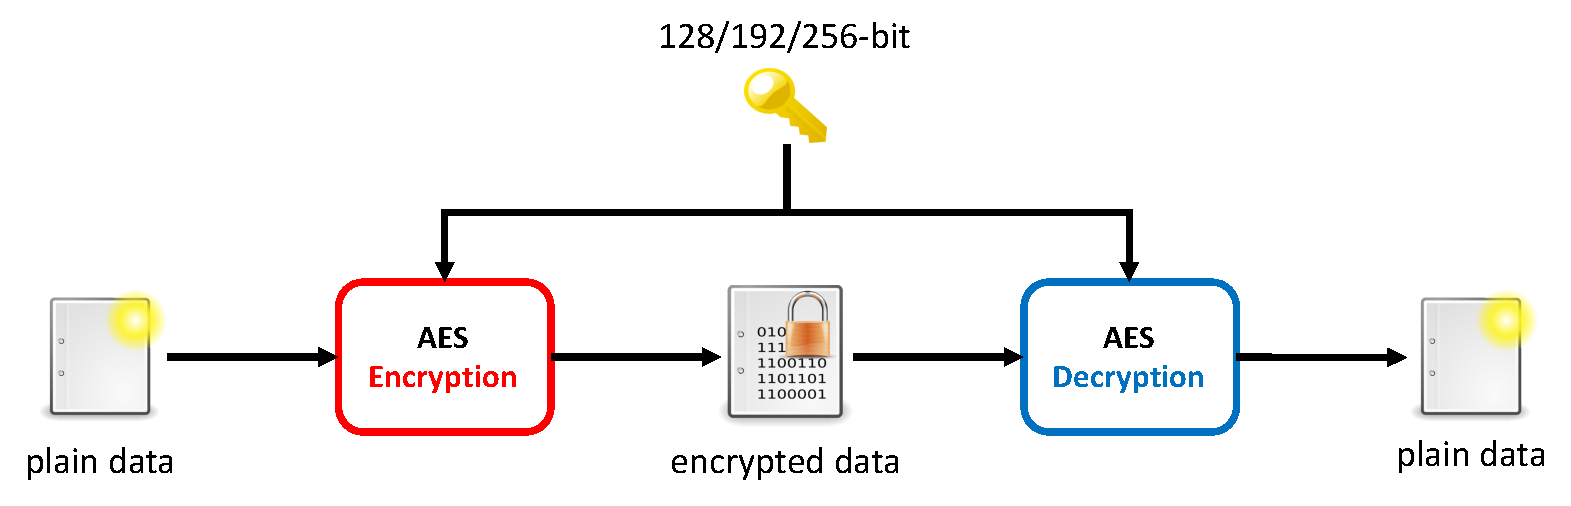
\includegraphics[width=0.9\linewidth]{Figs/aes_flow.pdf}
\end{center}
\end{frame}


\begin{frame}
\frametitle{AESを使うために}
AESを使う際に気をつけるお作法は、ざっと3点。
\begin{enumerate}
 \item AESで使う鍵の\alert{ランダム具合}
 \item AESで使う鍵を\alert{総当りする際の大変さ}\footnote[frame]{1点目と2点目は似ているようで異なる。}
 \item AESの\alert{利用モードの安全性}
\end{enumerate}

\vspace{2ex}
つまりどういうこと?

\end{frame}

\begin{frame}
\frametitle{準備: パスワードとかを使ったAES暗号化のポイント}
\begin{block}{\small パスワード $\neq$ AES暗号化の鍵}
パスワードやマスターシークレットを元にしてAES暗号化するためには、「パスワード等を変換し、AES暗号化の鍵を導出」することが必要
\end{block}
\begin{center}
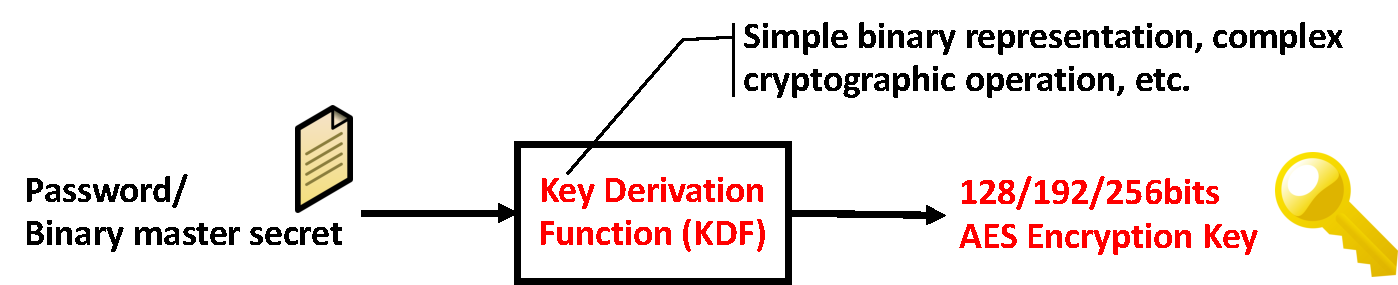
\includegraphics[width=\linewidth]{Figs/kdf_definition.pdf}
\end{center}
\end{frame}

\begin{frame}
\frametitle{1: AESで使う鍵のランダム具合?}
$\Rightarrow$ \alert{過去の利用履歴も含めたランダムさ}のこと

\vspace{1ex}

\begin{block}{}
つまり…
\begin{itemize}
\item 過去に暗号化に使った鍵は\alert{二度と使わない}
\item 暗号化の鍵は、過去の鍵から\footnote[frame]{および未来に使う鍵からも}は容易に導出できないものへと\alert{毎回ランダム変更}する
\end{itemize}
ということ。
\end{block}

\end{frame}

\begin{frame}
…なぜか?

$\Rightarrow$鍵が1つ漏れてしまうと、過去の暗号化データまで一網打尽…。

\begin{center}
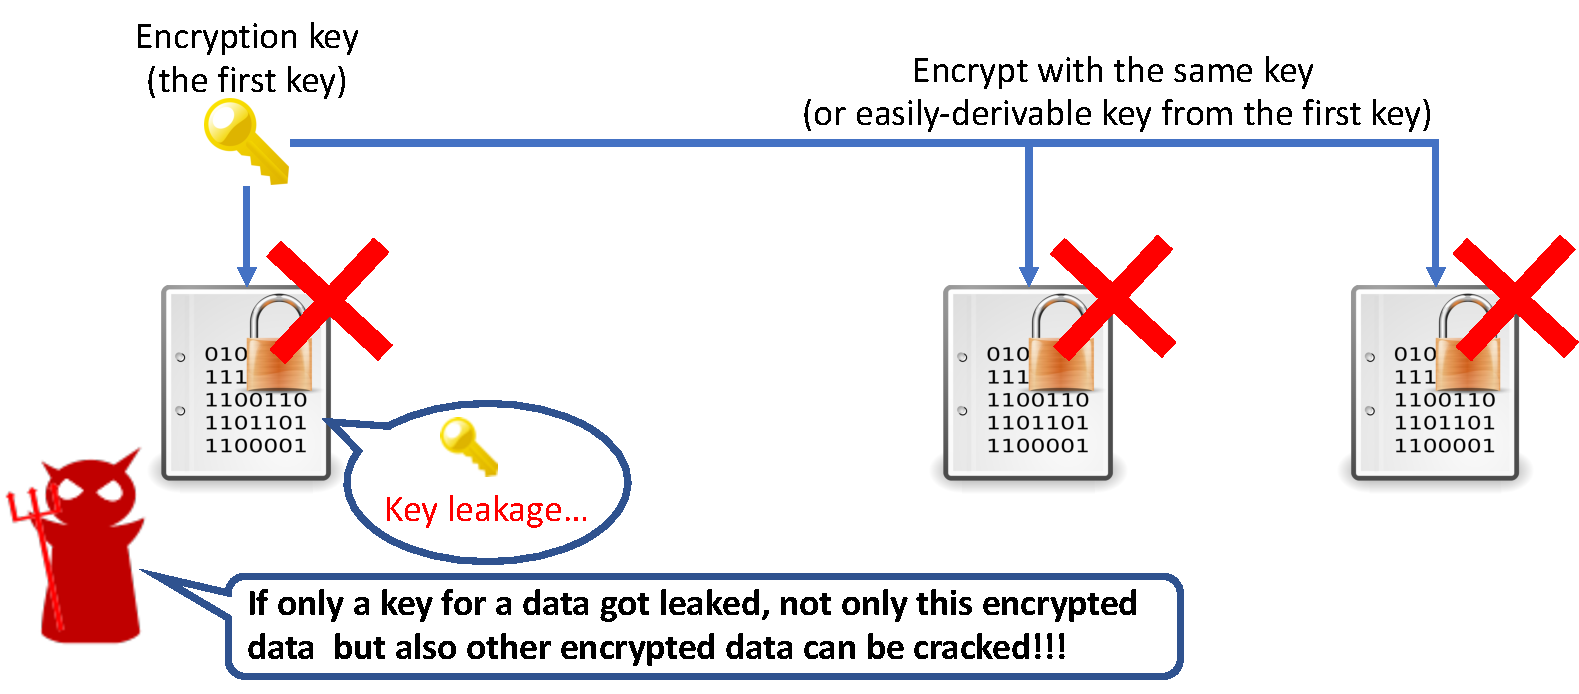
\includegraphics[width=0.9\linewidth]{Figs/pfs_bad_case.pdf}
\end{center}

\begin{block}{}
なので、万一鍵が1つ漏れちゃったとしても、他の暗号化データにまで影響が出ないことを保証しなきゃならない。
\end{block}

\end{frame}

\begin{frame}
だが、\underline{暗号化毎のパスワード等のランダム変更は非現実的}。

\vspace{2ex}

$\Rightarrow$ \alert{固定パスワード等からランダムに鍵を導出する方法}を使う\footnote[frame]{PBKDF2 (RFC8018), HKDF (RFC5869)}。

\begin{center}
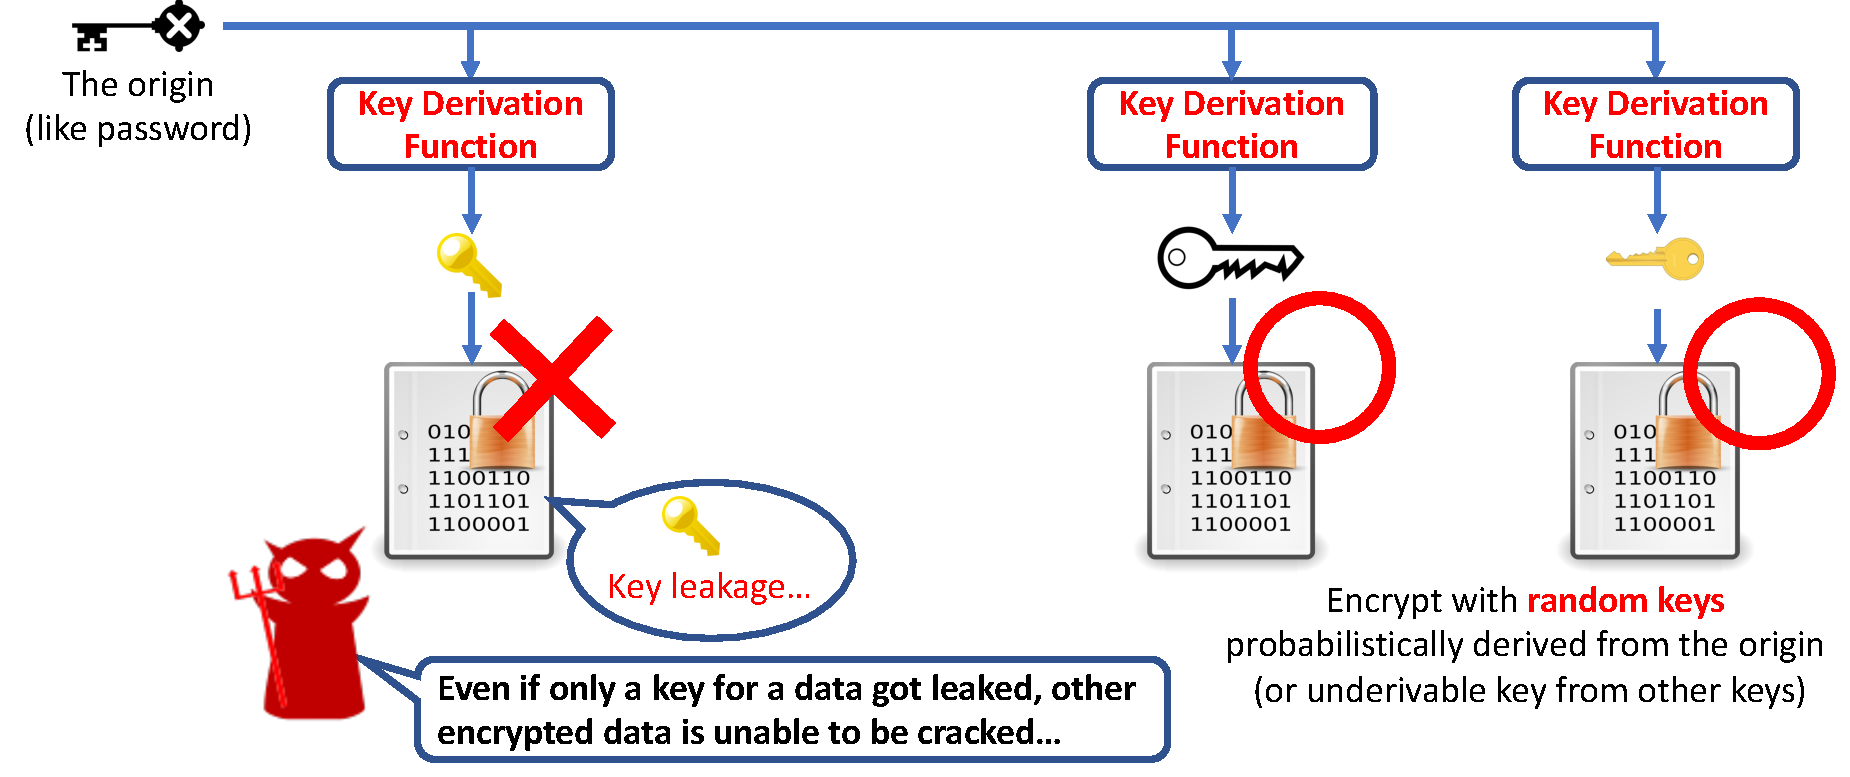
\includegraphics[width=0.9\linewidth]{Figs/pfs_kdf_case.pdf}
\end{center}

※ただし、固定パスワード等そのものが漏洩した場合はこの場合でもアウトなことに注意
\end{frame}

\begin{frame}
\frametitle{2: AESで使う鍵を総当りする際の大変さ?}

$\Rightarrow$ 総当たり攻撃のためのコストのこと。

\alert{※特にパスワードを使って暗号化する場合に重要}

\vspace{1ex}

\begin{block}{\small 暗号化データに対する総当たり攻撃}
鍵の候補を全通りを一覧で用意して、「当たり」を見つけるまでとにかく復号を繰り返すこと。
\end{block}

\vspace{2ex}

つまり総当たり攻撃のコストは、「ストレージ量」と「計算量」。

\alert{このコストを払うことが非現実的に高くなければヤバい。}
\end{frame}

\begin{frame}
\begin{block}{\small 8桁パスワードを単純にバイナリ化して鍵としてしまうと…}
大小英数字$8$桁パスワードは $62^8 < 2^{48}$ 通り。

\begin{itemize}
\item[$\Rightarrow$] $48$bitsの全通りの準備は、高々$1.5$PB。
\item[$\Rightarrow$] ストレージなしでも、パスワード候補を都度バイナリ化するだけで復号を試行可能。
\end{itemize}
\alert{割と簡単に「当たり=48bits」が見つかってしまう}。\footnote[frame]{\scriptsize 2009年当時でもスパコンを使って60時間とか。今だとGPUで並列化すればもっと高速になる。\url{https://web.archive.org/web/20180412051235/http://www.lockdown.co.uk/?pg=combi&s=articles}}
\end{block}
\vspace{1ex}

\begin{center}
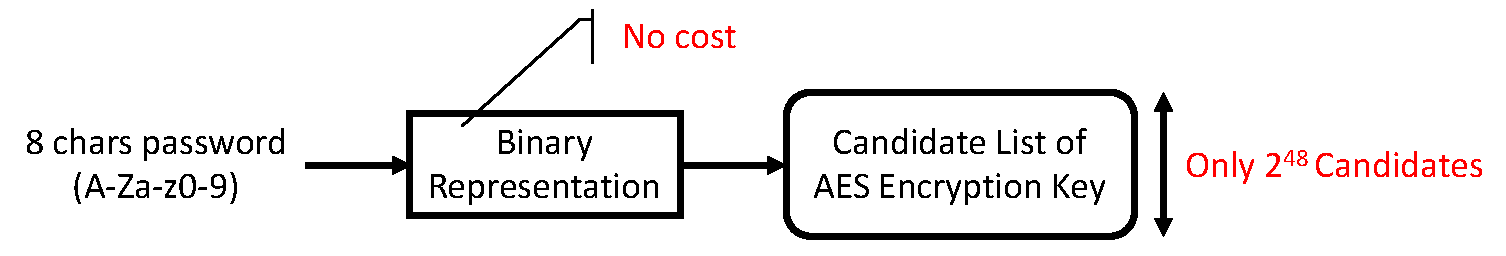
\includegraphics[width=0.9\linewidth]{Figs/kdf_weak.pdf}
\end{center}

\end{frame}

\begin{frame}

なので、短いパスワード等から鍵を作るときは、コストが膨大になるような変換をする。

\vspace{2ex}
\begin{block}{}
パスワード等から暗号化の鍵を作るとき、
\begin{itemize}
\item 毎回使い捨てのランダム値(Saltと呼ぶ)と混合して、\alert{AES暗号化の鍵のランダム性を上げる}。
\item \alert{計算コストの高い演算}を使う。
\end{itemize}
という処理を行う。\footnote[frame]{PBKDF2}
\end{block}

\begin{center}
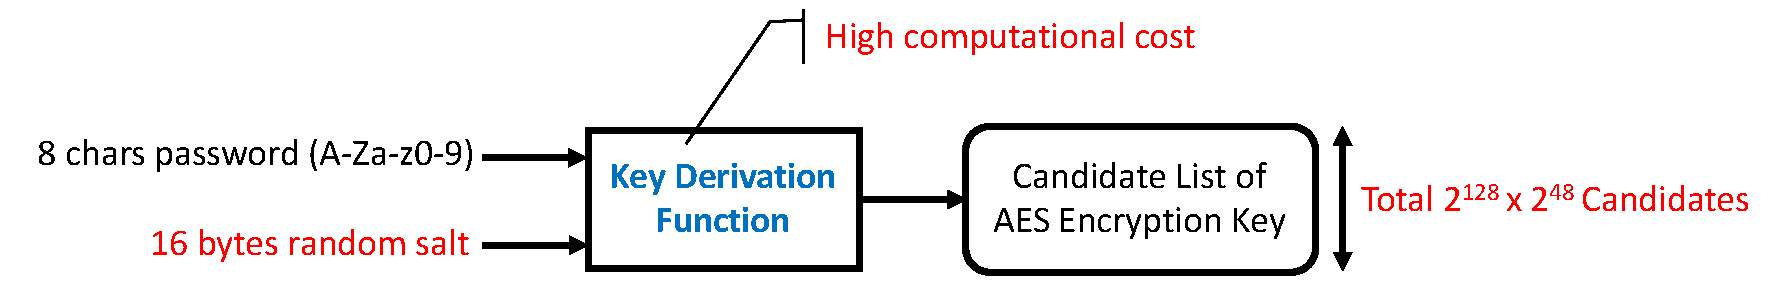
\includegraphics[width=\linewidth]{Figs/kdf_strong.pdf}
\end{center}

\end{frame}

\begin{frame}

\begin{center}
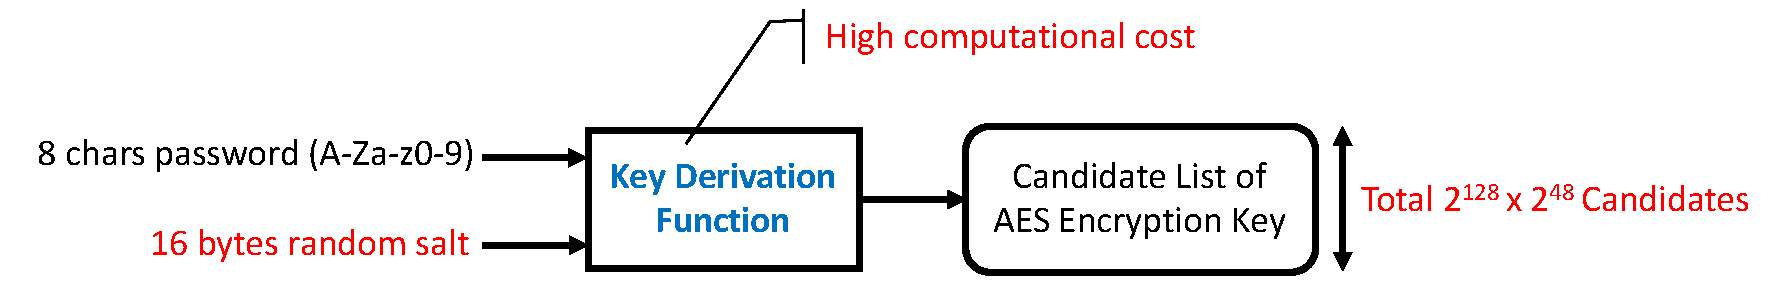
\includegraphics[width=\linewidth]{Figs/kdf_strong.pdf}
\end{center}

\begin{itemize}
 \item ランダムなSaltと混合することで、\alert{鍵候補全通りの事前準備のストレージが膨大になる}
 \item ストレージなしで試行しても、計算コストの高い演算のせいで、\alert{鍵候補を都度生成→復号の計算コストが莫大になる}
\end{itemize}

\vspace{2ex}

「お作法1」と合わせて1つの関数で実行することが多いが、AES暗号化の鍵を作る際に意識する重要なポイント。

\end{frame}


\begin{frame}
\frametitle{3: AESの利用モードの安全性?}

$\Rightarrow$ AESのAPIで設定できる利用モード('AES256-CBC'とか)と、そのパラメタの適切な設定をしないと\underline{致命的な事態に陥る}。

\vspace{2ex}

\begin{block}{\small AESの「利用モード」}
AESの処理1回で暗号化できるのはたった16bytesにすぎない。

長いデータを連続で暗号化するために、\alert{暗号化処理を連続して組み合わせる方法}が利用モード。
\end{block}

\end{frame}

\begin{frame}
\begin{block}{\small「とりあえずAESを使う」ための利用モード設定のポイントは2つ}
\begin{itemize}
\item 初期ベクトル(IV)というパラメタは\alert{都度ランダム値にする}\footnote[frame]{APIによって、ナンス(Nonce)というパラメタもあればそれも。}。
\item CTRモード・CBCモードあたりを使う。\alert{ECBモードは絶対に使わない。}
\end{itemize} 
\end{block}

前者、「過去に暗号化したデータとの相関をなくす」ために必要なパラメタ設定。

後者、\alert{ECBモードは論外} (これが言いたいこと)。
\end{frame}

\begin{frame}
どうしてECBモードは論外なのか?
\begin{itemize}
 \item[$\Rightarrow$] 元のデータの中で「同じ値のブロック\footnote[frame]{1ブロックは16Bytes単位}」は、暗号化データにおいても必ず「同じ値のブロック」になる。
 \item[$\Rightarrow$] \alert{暗号化されてても中のデータが何かというのが予測可能…}
\end{itemize}
\begin{center}
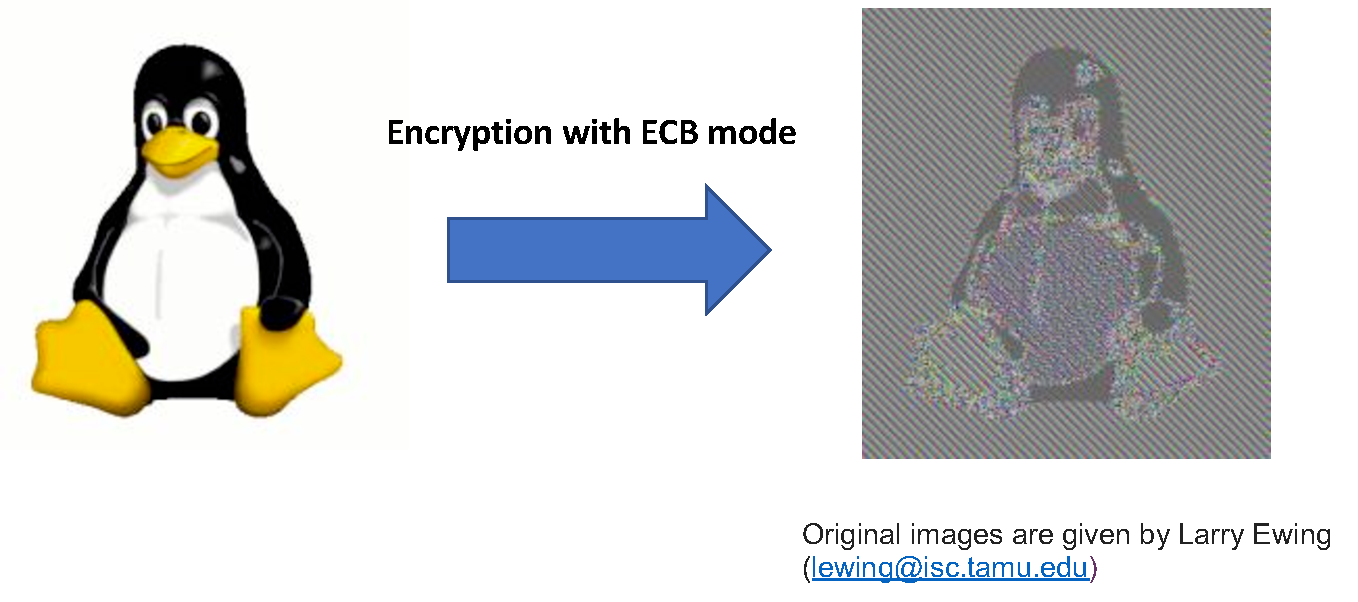
\includegraphics[width=0.8\linewidth]{Figs/ecb_mode.pdf}
\end{center}

というわけで、JavaScript以外でも、たとえ選べたとしても絶対にECBモードは利用してはいけない。
\end{frame}

\begin{frame}
ECBモードと違って、CBCモードではそういうことが起きない。
\begin{itemize}
 \item 先頭の16Bytesはランダムな初期化ベクトルと混ぜる
 \item 前の16Bytesの暗号化データを混ぜて次の16Bytesを処理
\end{itemize}

\vspace{2ex}

\begin{center}
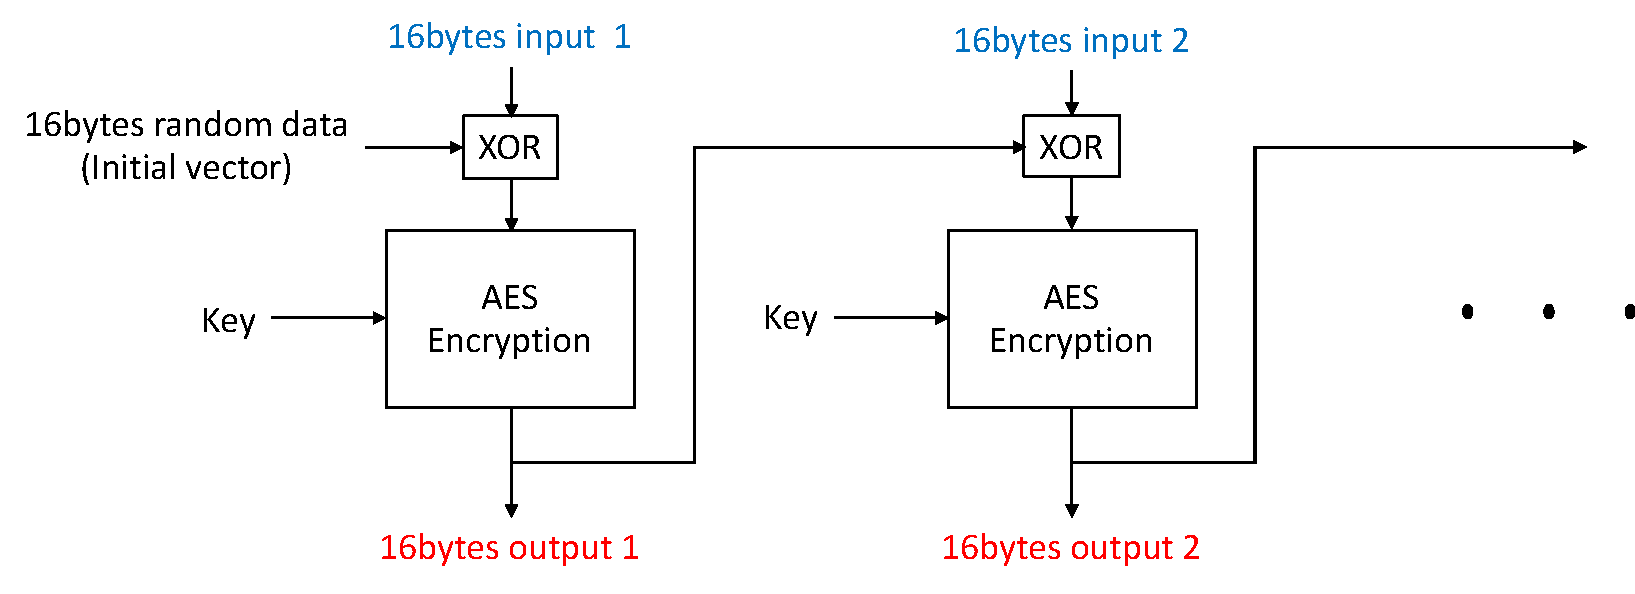
\includegraphics[width=0.8\linewidth]{Figs/cbc_mode.pdf}\\
CBCモードの16Bytes毎の処理
\end{center}
\end{frame}

%%%%%%%%%%%%%%%%%%%%%%%%%%%%%%%%%%%%%%%%%%%%%%%%%%%%%%%%%%%%%%%%%%%%%%%%%%%%%%%%%%%%%%%%%%%%%%%%%%%
\section{AESの使い方: とりあえず暗号化してみよう}
\begin{frame}
\centering
{\Large AESの使い方: とりあえず暗号化してみよう}
\end{frame}

\begin{frame}
\frametitle{今回のセッティング}
前回同様のREST APIサーバを介したE2E暗号化。
\begin{center}
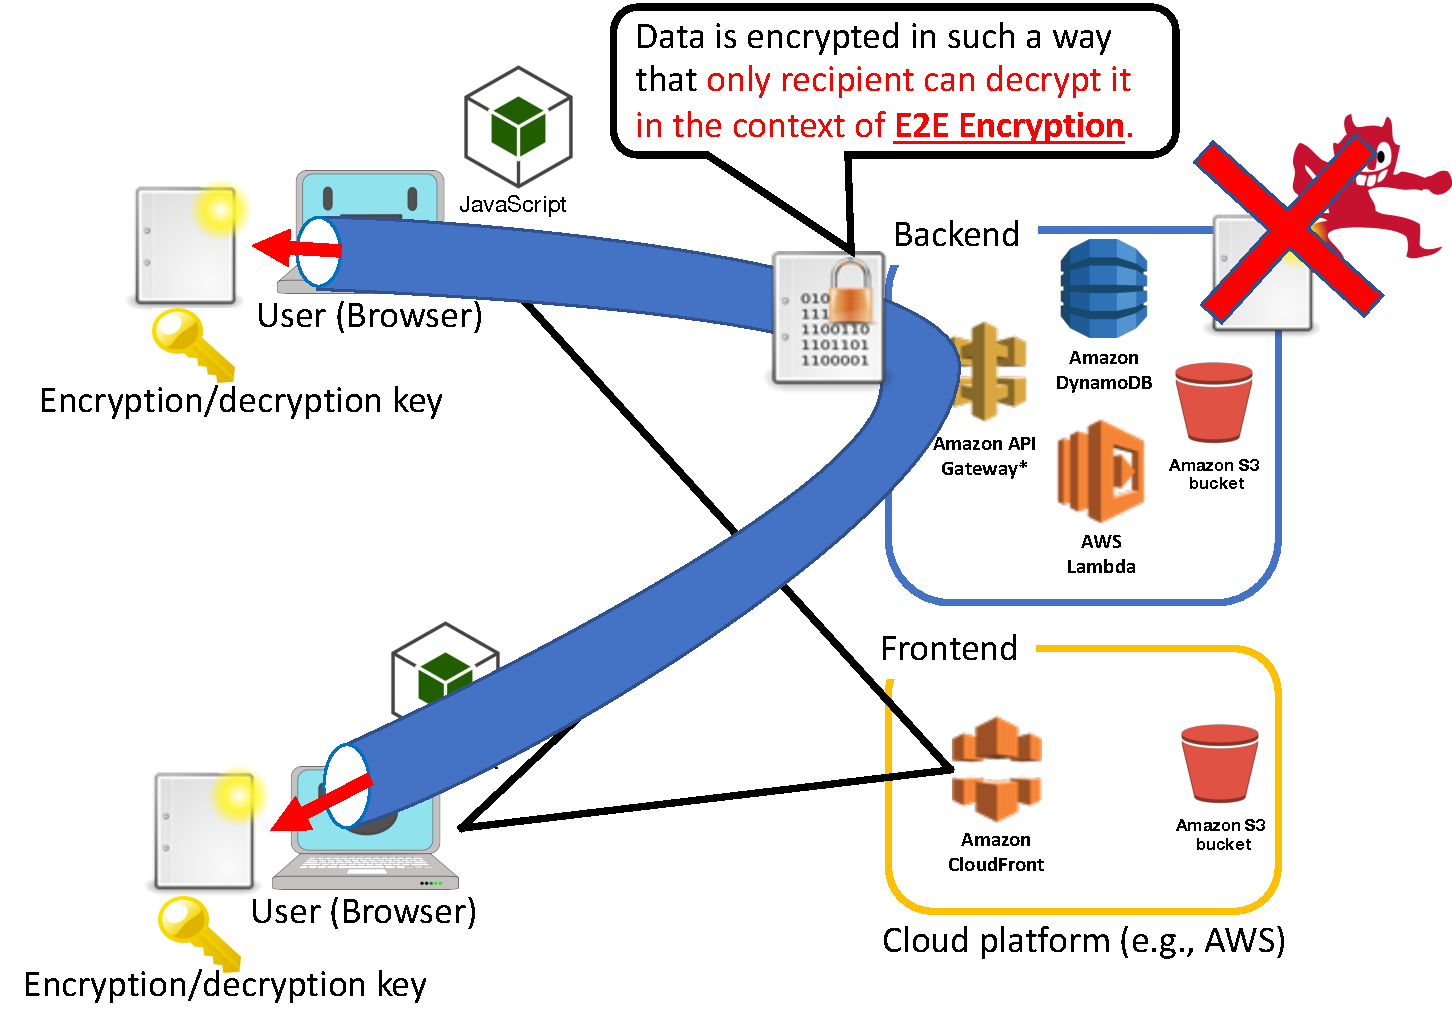
\includegraphics[width=0.9\linewidth]{Figs/e2e.pdf}
\end{center}
\end{frame}

\begin{frame}
ブラウザ・Node.jsをエンドとし、
\begin{enumerate}
 \item 「パスワード」「マスターシークレット」から鍵を導出し\footnote[frame]{お作法1,2}
 \item それを使ってAES-CBCモードで暗号化して\footnote[frame]{お作法3}
\end{enumerate}
REST APIで暗号化データを登録してみる。
\begin{center}
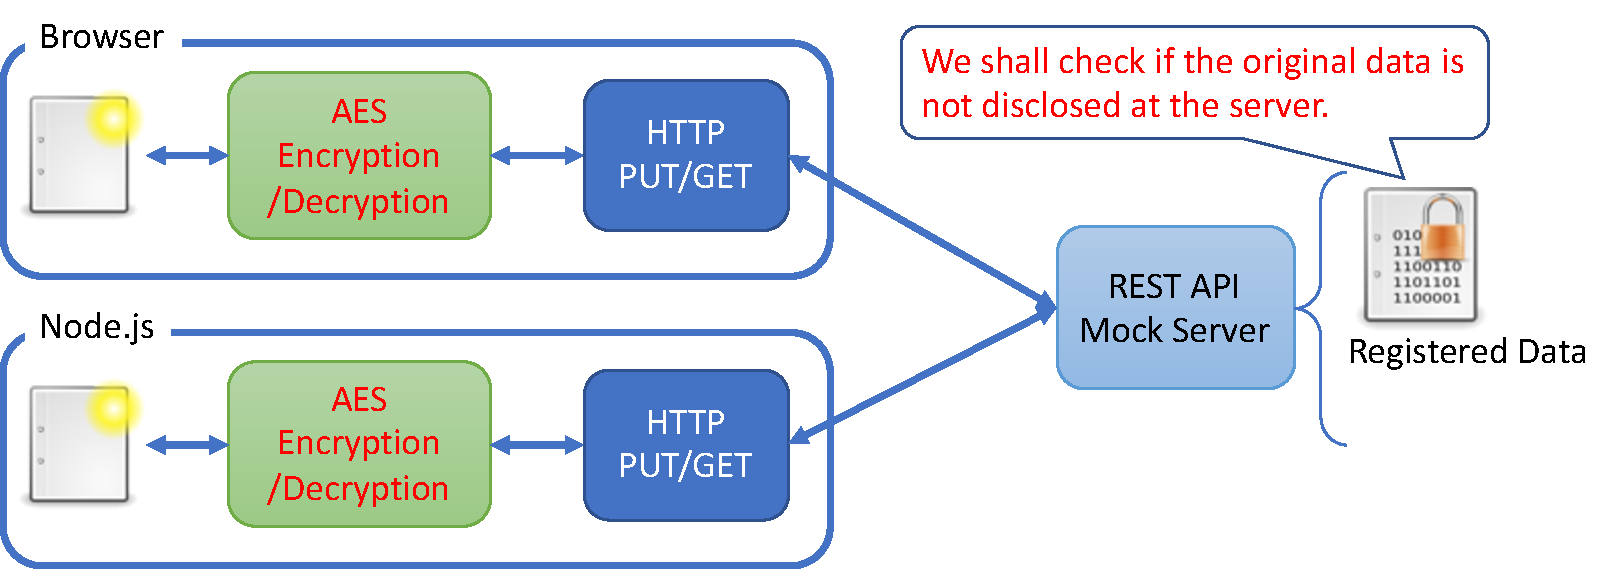
\includegraphics[width=\linewidth]{Figs/mock_flow.pdf}
\end{center}
\end{frame}

\begin{frame}
\frametitle{環境}
以下の環境が前提:
\begin{itemize}
 \item Node.js ($>$ v10)がインストール済。yarnが使えること。 \footnote[frame]{インストールコマンド: \texttt{npm i -g yarn}}
 \item ブラウザとして、Google Chrome (系ブラウザ)、もしくはFirefoxがインストール済み
 \item Visual Studio Code や WebStorm などの統合開発環境がセットアップ済みだとなお良い。
\end{itemize}
\end{frame}

\begin{frame}
\frametitle{JavaScriptプロジェクトの準備}
\begin{itemize}
\item プロジェクトのGitHubリポジトリ\footnote[frame]{\url{https://github.com/zettant/e2e-security-02}}をClone\\
\begin{exampleblock}{}
\footnotesize
\$ \texttt{git clone https://github.com/zettant/e2e-security-02}\\
\$ \texttt{cd e2e-security-02/sample}
\end{exampleblock}
\item 依存パッケージのインストール
\begin{exampleblock}{}
\$ \texttt{yarn install}
\end{exampleblock}
\item ライブラリのビルド
\begin{exampleblock}{}
\$ \texttt{yarn build}
\end{exampleblock}
\end{itemize}
\end{frame}

\begin{frame}
\frametitle{REST APIモックサーバの準備}
今回はSSL接続可能な共有サーバを準備済 (\url{https://e2e.zettant.com/})。

\vspace{2ex}

別途、検証用のサーバをローカルで立ち上げ可能。
\begin{exampleblock}{\small モックサーバの立ち上げ}
\$ \texttt{yarn start}
\end{exampleblock}
起動すると、localhostの3000番ポートでHTTPリクエストを待ち受け開始する。
\end{frame}

\begin{frame}
まずはコマンドラインを叩き、Node.jsで
\begin{itemize}
 \item パスワードでAES暗号化
 \item マスターシークレットでAES暗号化
 \item ヤバい利用モードでのヤバさを実感
\end{itemize}
してみる。

\vspace{2ex}

※ユニバーサル暗号ユーティリティ「jscu」\footnote[frame]{\url{https://github.com/junkurihara/jscu}}を使ってサンプルを制作しているので、\alert{ブラウザでも全く同じAPI・Code snippetを試用可能。}
\end{frame}

\begin{frame}
\frametitle{パスワードで暗号化してみる}
\small

「yarn execute post -r -p `パスワード' `データ'」で暗号化。

\begin{block}{\small sampleディレクトリ以下で実行}
\scriptsize
\$ \texttt{yarn execute post -r -p 'my password' 'my private data'} // -r を抜くとローカル\\
\texttt{Register encrypted data to remote server}\\
\texttt{Data: my private data}\\
\texttt{Password: my password}\\
{\color{red}
\texttt{Derived key and its related params:} // パスワードから生成された鍵とパラメタ\\
\texttt{\quad Derived key in Base64: fiP4flrlhd3Iwg5MOyln7zNNk4Au9If429n2uvfi43s=}\\
\texttt{\quad PBKDF2 Param - Salt in Base64: zyD7/TGDq3dig3l4zJ5SRzFKVnIjw2KG26XUrMZFkkw=}\\
\texttt{\quad PBKDF2 Param - Hash: SHA-256}\\
\texttt{\quad PBKDF2 Param - Iteration: 2048}
}\\
\texttt{Registered id: 1} // id=1で暗号化データと鍵導出のパラメタを登録
\end{block}

長い鍵「S4lFVWrvLj4OjPfFRTgVJFfRUI+6LIlw1VooFzG2J5E=」を短い「my password」から生成。

また、同じパスワード・データでも毎回異なる鍵になることを確認する。
\end{frame}

\begin{frame}
登録データは\url{https://e2e.zettant.com/data}で一覧。

\begin{center}
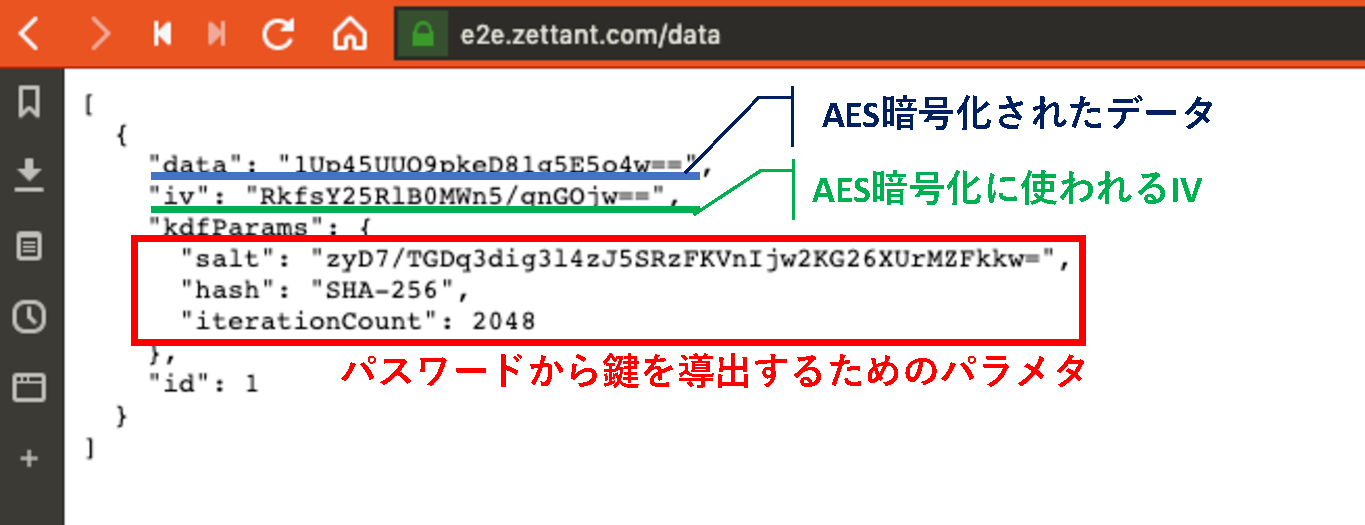
\includegraphics[width=\linewidth]{FigsSample02/data_pbes.pdf}
\end{center} 

暗号化データ以外、復号側と共有する公開パラメタ:
\begin{itemize}
 \item AESのCBCモード → IV
 \item パスワードから鍵の導出 → Salt, iteration回数、Hash関数
\end{itemize}
\end{frame}

\begin{frame}
 「yarn execute get -r -p `パスワード' `id番号'」で復号。
\begin{block}{}
\scriptsize
\$ \texttt{yarn execute get -r -p 'my password' 1} // -r を抜くとローカル\\
\texttt{Retrieve encrypted data to remote server}\\
\texttt{Id: 1}\\
\texttt{Password: my password}\\
{\color{blue}
\texttt{Derived key and its related params:} // 取得した公開パラメタと、生成した鍵\\
\texttt{\quad Derived key in Base64: fiP4flrlhd3Iwg5MOyln7zNNk4Au9If429n2uvfi43s=}\\
\texttt{\quad PBKDF2 Param - Salt in Base64: zyD7/TGDq3dig3l4zJ5SRzFKVnIjw2KG26XUrMZFkkw=}\\
\texttt{\quad PBKDF2 Param - Hash: SHA-256}\\
\texttt{\quad PBKDF2 Param - Iteration: 2048}\\
}
\texttt{Decrypted data: my private data} // 正しく復号された
\end{block}

暗号化の時と同一の鍵が生成されたことに注目。

\vspace{2ex}

中のコードがどうなっているかは後述。
\end{frame}


\begin{frame}
\frametitle{マスターシークレット(バイナリ)で暗号化してみる}
\small
「yarn execute post -r -m `マスターシークレット' `データ'」で暗号化。\footnote[frame]{マスターシークレットはBase64}

\begin{block}{\small sampleディレクトリ以下で実行}
\scriptsize
\$ \texttt{yarn execute gen-secret 32} // まずはBase64でマスターシークレットを生成する。\\
\texttt{Generated master secret in Base64: \alert{mP95WFEv3G/iWsjQKC4mEuEmCkiS8dRK80Q6CpC1bc0=}}\\[2ex]
\$ \texttt{yarn execute post -r -m 'mP95WFEv3G/iWsjQKC4mEuEmCkiS8dRK80Q6CpC1bc0=' 'my private data'}\\
\texttt{Register encrypted data to remote server}\\
\texttt{Data: my private data}\\
\texttt{Master secret: mP95WFEv3G/iWsjQKC4mEuEmCkiS8dRK80Q6CpC1bc0=}\\
{\color{red}
\texttt{Derived key and its related params:} // マスターシークレットから生成された鍵とパラメタ\\
\texttt{\quad Derived key in Base64: 1vgTfxp3FEi3kpJiQ6h0vxtDCkdz+u5XQUF1tPm1VMY=}\\
\texttt{\quad HKDF Param - Salt in Base64: 8SM9tyXJUX+JGwLswIUnnGyHPL+7hzkSHXaKY7z0AF0=}\\
\texttt{\quad HKDF Param - Hash: SHA-256}
}\\
\texttt{Registered id: 2}
\end{block}

同じマスターシークレット・データでも毎回異なる鍵になることを確認する。

\end{frame}


\begin{frame}
ブラウザで確認してみる。

\begin{center}
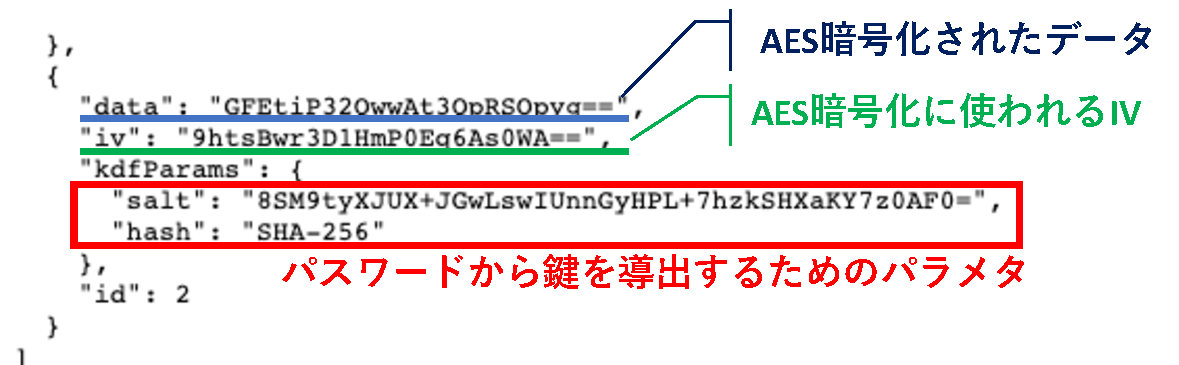
\includegraphics[width=\linewidth]{FigsSample02/data_hkdf.pdf}
\end{center} 

暗号化データ以外、復号側と共有する公開パラメタ:
\begin{itemize}
 \item AESのCBCモード → IV
 \item マスターシークレットから鍵の導出 → Salt, Hash関数
\end{itemize}
\end{frame}

\begin{frame}
 「yarn execute get -r -m `マスターシークレット' `id番号'」で復号。
\begin{block}{}
\scriptsize
\$ \texttt{yarn execute get -r -m 'mP95WFEv3G/iWsjQKC4mEuEmCkiS8dRK80Q6CpC1bc0=' 2} // -r を抜くとローカル\\
\texttt{Retrieve encrypted data to remote server}\\
\texttt{Id: 2}\\
\texttt{Master secret: mP95WFEv3G/iWsjQKC4mEuEmCkiS8dRK80Q6CpC1bc0=}\\
{\color{blue}
\texttt{Derived key and its related params:} // 取得した公開パラメタと、生成した鍵\\
\texttt{\quad Derived key in Base64: 1vgTfxp3FEi3kpJiQ6h0vxtDCkdz+u5XQUF1tPm1VMY=}\\
\texttt{\quad HKDF Param - Salt in Base64: 8SM9tyXJUX+JGwLswIUnnGyHPL+7hzkSHXaKY7z0AF0=}\\
\texttt{\quad HKDF Param - Hash: SHA-256}}
\\
\texttt{Decrypted data: my private data} // 正しく復号された
\end{block}

暗号化の時と同一の鍵が生成されたことに注目。

\vspace{2ex}

中のコードがどうなっているかは後述。
\end{frame}


\begin{frame}
ブラウザでもパスワード暗号化・マスターシークレットでの暗号化が試せる。

\vspace{1ex}

\texttt{sample02/src/post-get-browser.html} を開いて開発者コンソールから試してみよう。

\vspace{1ex}

(サンプルコードはhtmlファイルに記載)
\end{frame}

\begin{frame}
\frametitle{危ない暗号化モードで暗号化してみる}
ECBモードで暗号化できるAPIを用意してみたので、それで暗号化してみるとヤバさが目に見えてわかる。

\begin{exampleblock}{}
\scriptsize
\$ \texttt{yarn execute aes-mode-compare '\alert{0123456789ABCDEF}\structure{0123456789ABCDEF}'} ←16bytes毎\\
\texttt{random key (Base64): 4gfrl+/OMyFt2ALLEp24sIXyHsyjvlYZZxRj4lkJe9M=}\\
\texttt{data (Hex): 3031323334353637383941424344454630313233343536373839414243444546}\\
\texttt{AES-ECB (Hex): \underline{\alert{c871e345b92951236059676b0866c7af}} \underline{\structure{c871e345b92951236059676b0866c7af}} ...}\\
\texttt{AES-CBC (Hex): \alert{d34ad4cc8816edcf3ad1a56c355c9067} \structure{69c4f525903b607960e377649abef648} ...}
\end{exampleblock}

16bytes単位で同じ値が出てくるデータを、ECBモードで暗号化してみると\alert{ECBモードだと暗号文も同じ値の繰り返しになる}。\\
$\Rightarrow$ \underline{元のデータが推測しやすくなる。}

\end{frame}

\begin{frame}
CBCモードだと暗号化データが繰り返されるようなことはない。\footnote[frame]{というか、繰り返しが発生してしまうようなものはECBだけ。}

\vspace{3ex}
ECBモードについては、WebCryptoAPIなどではその危険性のためにサポートされていない\footnote[frame]{サンプルコードでは、CBCモードを弄ってECBモードを再現している。}が、\alert{どんな場合であってもECBモードの利用は避けて}、CBCモードやCTRモードなどを利用しよう。
\end{frame}


%%%%%%%%%%%%%%%%%%%%%%%%%%%%%%%%%%%%%%%%%%%%%%%%%%%%%%%%%%%%%%%%%%%%%%%%%%%%%%%%%%%%%%%%%%%%%%%%%%%
\section{AESの使い方: 細かめの解説}
\begin{frame}
\centering
{\Large AESの使い方: 細かめの解説}
\end{frame}

\begin{frame}
\frametitle{PBKDF2の使い方 in JavaScript}
パスワードからAESの鍵を導出するのに使った。
\begin{block}{\small PBKDF2: Password-based Key Derivation Function}
PKCS \#5 v2.1 (RFC8081\footnote[frame]{\scriptsize \url{https://tools.ietf.org/html/rfc8018}}) にて規定。
非推奨のPBKDF1の置き換え。PBKDF2 を利用した(AES)暗号化は、Password-based Encryption Scheme 2 (PBES2) と規定される。
\end{block}

\begin{center}
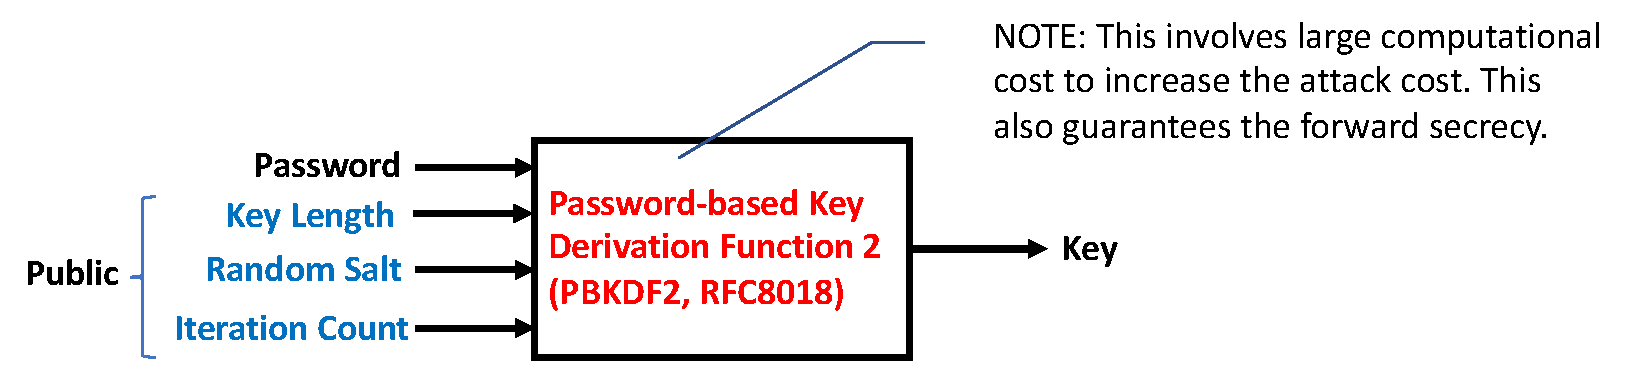
\includegraphics[width=\linewidth]{Figs/kdf_pbkdf2_flow.pdf}
\end{center}
他にも、BCryptなど類似のアルゴリズムがある。\footnote[frame]{\scriptsize 「パスワードハッシュ化」と「パスワードから鍵導出」で目的は異なれど、必要な機能は一緒。}
\end{frame}

\begin{frame}[fragile]
PBKDF2は、WebCrypto API, Node.js Crypto共にネイティブ実装。

今回は、手前味噌だがAPI差をなくすのに\texttt{jscu}を利用。

\begin{exampleblock}{\small \texttt{sample/src/derive-key.js: deriveKeyFromPassword}}
\scriptsize
\begin{verbatim}
const jscu = getJscu(); // 環境に応じてjscuをscriptタグで読み込んだり、requireしたり。

if(!salt){ // saltが入力されなかったらランダム値を生成。Saltは任意長。
  salt = jscu.random.getRandomBytes(32); // Uint8Array
}
else {
  salt = jseu.encoder.decodeBase64(salt); // Base64からUint8Arrayにデコード
}

const key = await jscu.pbkdf.pbkdf2( // PBKDF2により鍵導出
  password,       // パスワード。
  salt,           // 復号側と共有(公開)。
  iterationCount, // 内部処理の反復回数。通常1000回以上。復号側と共有(公開)。
  len,            // 出力する鍵の長さ。復号側と共有(公開)。
  hash            // 内部のHMAC関数用のHash関数名。'SHA-256'。復号側と共有(公開)。
);
\end{verbatim}
\end{exampleblock}
\end{frame}

\begin{frame}
\frametitle{HKDFの使い方 in JavaScript}
マスターシークレットからAESの鍵を導出するのに使った。
\begin{block}{\small HKDF: HMAC-based Key Derivation Function}
RFC8081\footnote[frame]{\scriptsize \url{https://tools.ietf.org/html/rfc5869}} にて規定。
PBKDF2と違って、\structure{鍵の導出計算量を莫大にする効果は薄い}ので、長めのマスターシークレットを元にする場合に使う。
\end{block}

\begin{center}
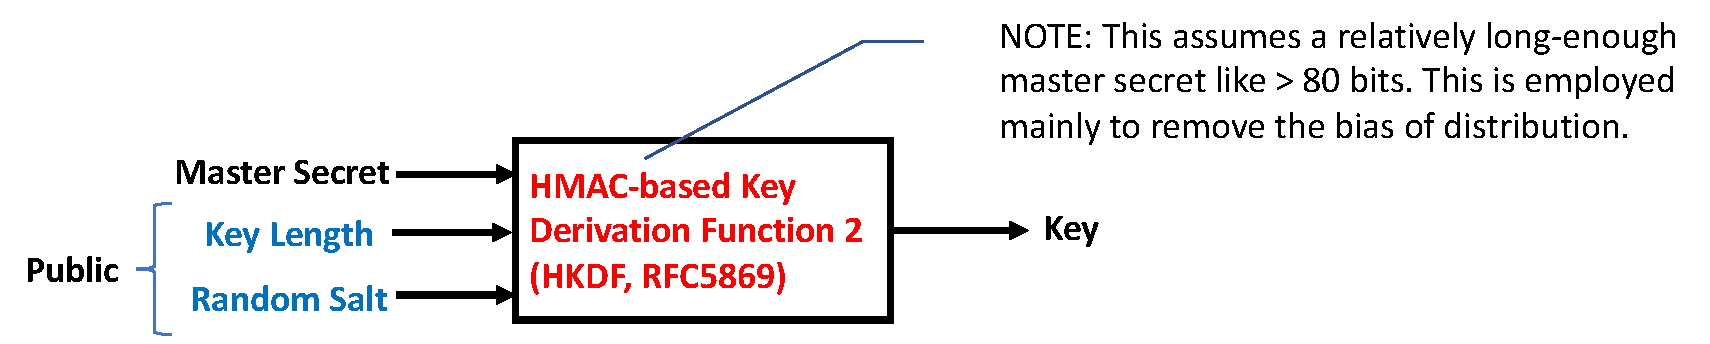
\includegraphics[width=\linewidth]{Figs/kdf_hkdf_flow.pdf}
\end{center}
\end{frame}

\begin{frame}[fragile]
HKDFは、WebCrypto APIでのみネイティブ実装。

今回は、手前味噌だが環境差をなくすのに\texttt{jscu}を利用。

\begin{exampleblock}{\small \texttt{sample/src/derive-key.js: deriveKeyFromMasterSecret}}
\scriptsize
\begin{verbatim}
const jscu = getJscu(); // 環境に応じてjscuをscriptタグで読み込んだり、requireしたり。

if(!salt){ // saltが入力されなかったらランダム値を生成。Saltは任意長。
  salt = jscu.random.getRandomBytes(32); // Uint8Array
}
else {
  salt = jseu.encoder.decodeBase64(salt); // Base64からUint8Arrayにデコード。
}

const keyObj = await jscu.hkdf.compute(
  masterSecret, // マスターシークレット。
  hash          // 内部のHMAC関数用のHash関数名。'SHA-256'。復号側と共有(公開)。
  len,          // 出力する鍵の長さ。復号側と共有(公開)。
  '',           // 'info' field for RFC5869. This could be always blank.
  salt          // 復号側と共有(公開)。
);
\end{verbatim}

\end{exampleblock}
\end{frame}

\begin{frame}[fragile]
\frametitle{暗号化モードの設定}
\texttt{jscu}では、CBCモードとCTRモードに加えて、CTRモードを拡張したGCM\footnote[frame]{\scriptsize GCM(Galois/Counter Mode)は、CTRモードで暗号化したデータに\structure{認証タグ}を付与したもの。暗号化したデータの改ざんを検知できる。}をサポートしている。

\begin{exampleblock}{\small \texttt{sample/src/encrypt.js: encrypt}}
\scriptsize
\begin{verbatim}
const jscu = getJscu(); // 環境に応じてjscuをscriptタグで読み込んだり、requireする。

const uint8iv = jscu.random.getRandomBytes(16); // ランダムIVの生成。CBCは16Bytes。
const encrypted = await jscu.aes.encrypt( // AES暗号化
  jseu.encoder.stringToArrayBuffer(data), // string dataのUint8Array化
  key,                                    // HKDF/PBKDFで導出した鍵
  { // CBC暗号化モードを設定
    name: 'AES-CBC',
    iv: uint8iv
  }
);
\end{verbatim}
\end{exampleblock}
\end{frame}

\begin{frame}[fragile]
\begin{exampleblock}{\small \texttt{sample/src/encrypt.js: decrypt}}
\scriptsize
\begin{verbatim}
const jscu = getJscu(); // 環境に応じてjscuをscriptタグで読み込んだり、requireする。

const decrypted = await jscu.aes.decrypt( // AES復号
  jseu.encoder.decodeBase64(data), // Base64の暗号化データをデコード。
  key,                             // HKDF/PBKDFで導出した鍵
  { // CBC暗号化モードを設定
    name: 'AES-CBC',
    iv: jseu.encoder.decodeBase64(iv) // Base64で与えられたIVをデコード。
  }
);
\end{verbatim}
\end{exampleblock}
\end{frame}



%%%%%%%%%%%%%%%%%%%%%%%%%%%%%%%%%%%%%%%%%%%%%%%%%%%%%%%%%%%%%%%%%%%%%%%%%%%%%%%%%%%%%%%%%%%%%%%%%%%
\section{まとめ}
\begin{frame}
 \centering
 {\Large まとめ}
\end{frame}

\begin{frame}
\frametitle{まとめ}
お疲れ様でした。

\begin{itemize}
\item AES暗号化する際のお作法を学んだ。
\begin{itemize}
 \item 鍵のランダムさを上げる、鍵への攻撃を困難にするためにKey Derivation Functionを適切に使う。\\
(※今回紹介したPBKDF2/HKDF以外の方法もある。\footnote[frame]{\scriptsize e.g., JOSE向けのConcat KDF with AESKW \url{https://tools.ietf.org/html/rfc8037}})
 \item 利用モードはCBCモードやCTRモードを使う。
\end{itemize}
\item お作法を守ったJavaScriptでの実装例を触ってみた。
\end{itemize}
\end{frame}

\begin{frame}
\frametitle{次回は}
\begin{itemize}
 \item 内容: 
\begin{itemize}
 \item 公開鍵暗号を使うコツ(数学的なことはやらない)
 \item RSA-OAEP
 \item EDCH-Ephemeral + AES
\end{itemize}
 \item 日時: 2019年10月17日(木曜日) 19:00- (2週間後)
 \item 場所: ブロックチェーンハブ (ここ)
 \item 発表者: (また) 栗原
\end{itemize}
\end{frame}


\begin{frame}
\frametitle{宣伝: iTransfy by Zettant}
\begin{center}
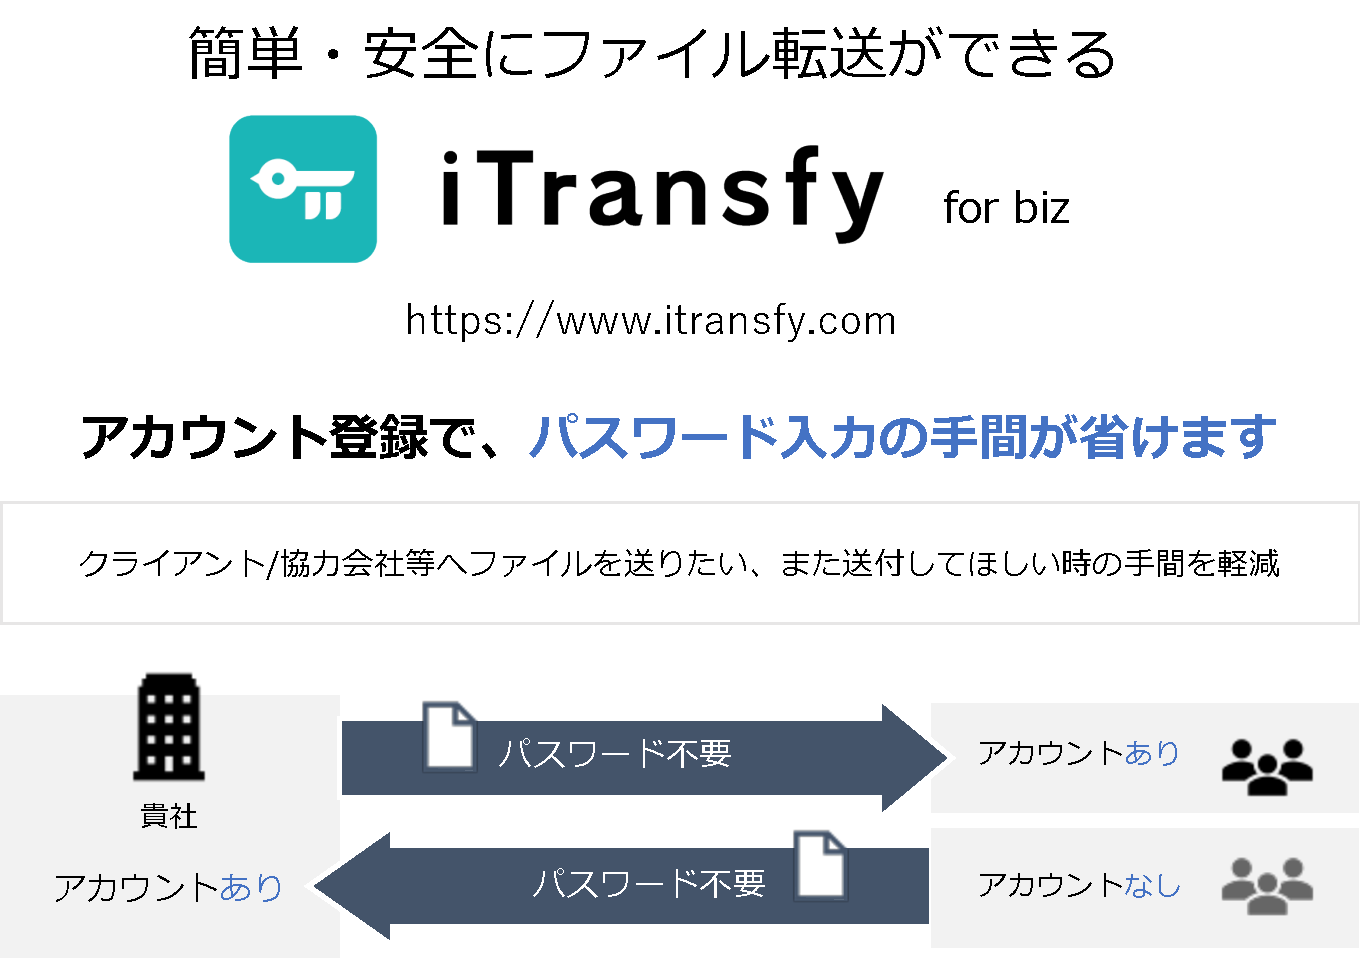
\includegraphics[width=0.9\linewidth]{FigsZettant/itransfy.pdf} 
\end{center}
\end{frame}

\begin{frame}
\frametitle{宣伝: 株式会社ゼタント}
\begin{tabular}{cc}
\begin{minipage}[b]{0.3\linewidth}

\includegraphics[width=\linewidth]{FigsZettant/logo.pdf}
\vspace{1ex}
\end{minipage}
 & 
\begin{minipage}[b]{0.7\linewidth}
\footnotesize
ゼタントはのミッションは、\\

「自分の身は自分で守ることができる世の中にする」\\

ことです。\\
共感してくれる仲間を募集しています!\\

問合せ先: \url{recruit@zettant.com}\\
会社URL: \url{https://www.zettant.com}
\end{minipage}
\end{tabular}
\end{frame}


% \begin{frame}
% 次回以降…リクエスト次第ですが、
% \begin{itemize}
% \item 公開鍵暗号とその使い方
% \item 「情報が改ざんされてない」ことを保証するために(電子署名とMAC)
% \item RFCとアルゴリズム・フォーマット
% \end{itemize}
% などを予定。
% \end{frame}


%%%%%%%%%%%%%%%%%%%%%%%%%%%%%%%%%%%%%%%%%%%%%%%%%%%%%%%%%%%%%%%%%%%%%%%%%%%%%%%%%%%%%%%%%%%%%%%%%%%

% \backupbegin
% \section{Backup}

% \begin{frame}
 
% \end{frame}

% \begin{frame}
%  \begin{enumerate}
%   \item 今回は共通鍵暗号
%   \item 公開鍵暗号\& Hybrid Encryption
%   \item ハッシュ・署名とHMAC
%  \item 超マニアック講座:RFCとアルゴリズム・フォーマット
%  \end{enumerate}
% \end{frame}

% \begin{frame}
% \frametitle{Appendix}
% This page is not counted.
% \end{frame}
% \backupend

\end{document}
%%%%%%%%%%%%%%%%%%%%%%%%%%%%%%%%%%%%%%%%%%%%%%%%%%%%%%%%%%%%%%%%%%%%%%%%%%%%%%%%%%%%%%%%%%%%%%%%%%%
%%%%%%%%%%%%%%%%%%%%%%%%%%%%%%%%%%%%%%%%%%%%%%%%%%%%%%%%%%%%%%%%%%%%%%%%%%%%%%%%%%%%%%%%%%%%%%%%%%%
%%%%%%%%%%%%%%%%%%%%%%%%%%%%%%%%%%%%%%%%%%%%%%%%%%%%%%%%%%%%%%%%%%%%%%%%%%%%%%%%%%%%%%%%%%%%%%%%%%%
%%%%%%%%%%%%%%%%%%%%%%%%%%%%%%%%%%%%%%%%%%%%%%%%%%%%%%%%%%%%%%%%%%%%%%%%%%%%%%%%%%%%%%%%%%%%%%%%%%%
%%%%%%%%%%%%%%%%%%%%%%%%%%%%%%%%%%%%%%%%%%%%%%%%%%%%%%%%%%%%%%%%%%%%%%%%%%%%%%%%%%%%%%%%%%%%%%%%%%%
%%%%%%%%%%%%%%%%%%%%%%%%%%%%%%%%%%%%%%%%%%%%%%%%%%%%%%%%%%%%%%%%%%%%%%%%%%%%%%%%%%%%%%%%%%%%%%%%%%%
